\chapter{Results}
\label{chap:results}

One can compare measured \RAA with the theory predictions \cite{RAA_prediction}. Values shown in the Figure~\ref{fig:RAA_prediction} were extracted by a 'data thief' and interpolated linearly between \sqn = 5.02 and 7.0 TeV. The analysis team is in contact with the authors of this paper to obtain the precise values of the suppression prediction done for \sqn = 5.02 TeV and the prediction for the no-quenching baseline. We have also requested the \pT range to be lowered below 10 GeV in the recalculation to \sqn = 5.36 TeV. Moreover, at least for the no-quenching baseline, authors of \cite{RAA_prediction_6p8} explicitly claim that the baseline is the same for \OO and \NeNe, which should be enough to put measured \RAA into a context. The theory group around Aleksas Mazeliauskas has also provided us with such a preliminary no-quenching prediction in the expected kinematic reach, shown in the Figure~\ref{fig:RAA_no_quench}. 

\begin{figure}[h]
    \centering
    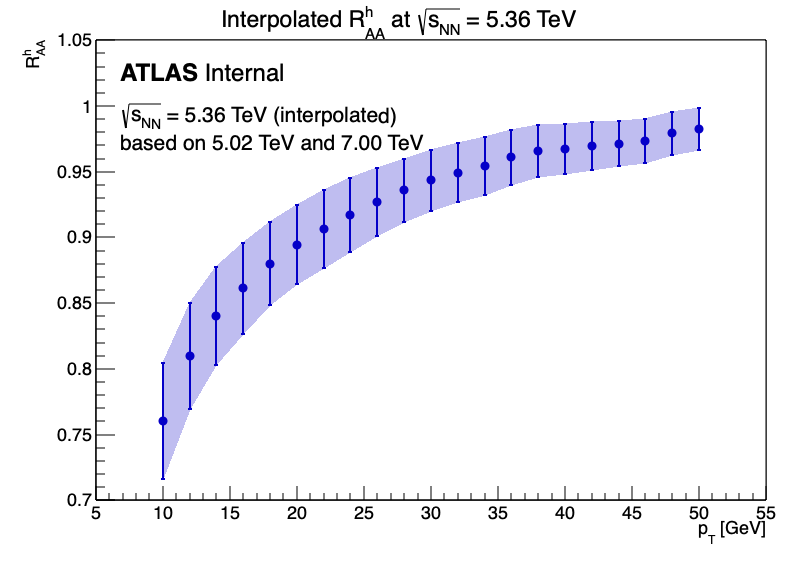
\includegraphics[width=0.7\linewidth]{images/RAA_prediction.png}
    \caption{\RAA prediction based on \cite{RAA_prediction}.}
    \label{fig:RAA_prediction}
\end{figure}

\begin{figure}[h]
    \centering
    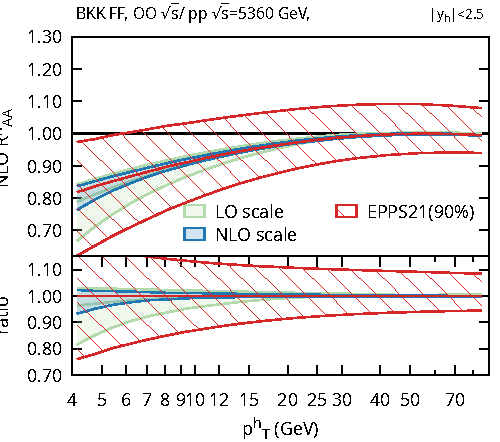
\includegraphics[width=0.7\linewidth]{images/plot_LHC_hadron_OO_RAA_90.pdf}
    \caption{No-quenching \RAA prediction valid both for \OO and \NeNe}
    \label{fig:RAA_no_quench}
\end{figure}